% Intended LaTeX compiler: pdflatex
\documentclass[11pt]{article}
\usepackage[utf8]{inputenc}
\usepackage[T1]{fontenc}
\usepackage{graphicx}
\usepackage{longtable}
\usepackage{wrapfig}
\usepackage{rotating}
\usepackage[normalem]{ulem}
\usepackage{amsmath}
\usepackage{amssymb}
\usepackage{capt-of}
\usepackage{hyperref}
\author{Construção de compiladores I}
\date{}
\title{Apresentação da disciplina}
\hypersetup{
 pdfauthor={Construção de compiladores I},
 pdftitle={Apresentação da disciplina},
 pdfkeywords={},
 pdfsubject={},
 pdfcreator={Emacs 29.4 (Org mode 9.7.22)}, 
 pdflang={English}}
\begin{document}

\maketitle
\section*{Objetivos}
\label{sec:org45f2319}

\subsection*{Objetivos}
\label{sec:org441fd78}

\begin{itemize}
\item Apresentar a importância da construção de compiladores na formação de um cientista da computação.
\item Apresentar a ementa, critérios de avaliação e bibliografia da disciplina.
\end{itemize}
\subsection*{Objetivos}
\label{sec:orga25ee60}

\begin{itemize}
\item Apresentar a visão geral de um compilador.
\end{itemize}
\section*{Compiladores}
\label{sec:org495af10}

\subsection*{Como executamos programas?}
\label{sec:orgd486270}
\begin{itemize}
\item Três técnicas principais
\begin{itemize}
\item Interpretação
\item Compilação
\item Virtualização.
\end{itemize}
\end{itemize}
\subsection*{Interpretação}
\label{sec:orgad50083}

\begin{itemize}
\item Código fonte é representado como uma estrutura de dados e
o intepretador executa o programa diretamente.
\item Interpretador é responsável pela execução do programa e de
sua interação com o S.O.
\end{itemize}
\subsection*{Compilação}
\label{sec:org9b5ad72}

\begin{itemize}
\item Código fonte é traduzido para uma nova linguagem.
\item Código alvo pode ser uma linguagem de alto nível (transpilação).
\item Código alvo pode ser uma linguagem de baixo nível (compilação).
\end{itemize}
\subsection*{Virtualização}
\label{sec:orgeb73b4e}

\begin{itemize}
\item Código fonte é traduzido para uma linguagem de baixo nível, não diretamente entendida
pelo hardware.
\item Normalmente, chamado de bytecode.
\item Intepretadores mais eficientes.
\end{itemize}
\section*{Visão geral (montanha)}
\label{sec:org3d542ea}

\begin{center}
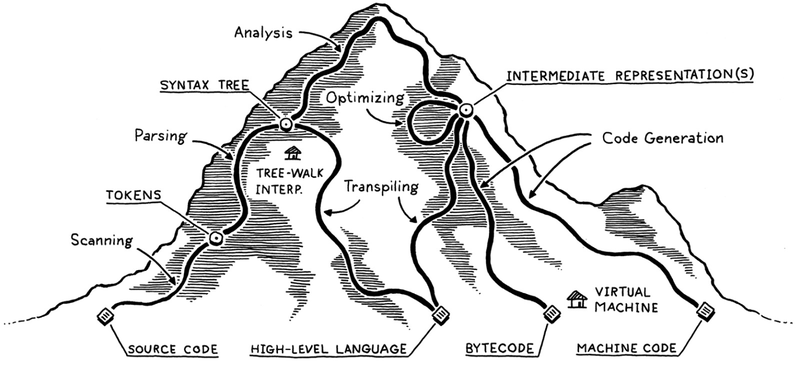
\includegraphics[width=.9\linewidth]{ montain.png}
\end{center}
\subsection*{Escalando a montanha}
\label{sec:orga0adf02}

\begin{itemize}
\item Análise Léxica: Dividir o código em \textbf{\textbf{tokens}}.
\begin{itemize}
\item Eliminar comentários e espaços em branco.
\end{itemize}
\end{itemize}
\subsection*{Escalando a montanha}
\label{sec:org74ab40b}

\begin{itemize}
\item Análise sintática: Organiza a sequência de tokens em sua estrutura gramatical.
\begin{itemize}
\item Produz uma árvore de sintaxe abstrata.
\end{itemize}
\end{itemize}
\subsection*{Escalando a montanha}
\label{sec:org1f058f2}

\begin{itemize}
\item Análise semântica: Verifica se a árvore produzida pelo analisador sintático atende restrições semânticas.
\begin{itemize}
\item Todos os símbolos foram declarados?
\item Argumentos de funções possuem a aridade e tipo corretos?
\end{itemize}
\end{itemize}
\subsection*{Escalando a montanha}
\label{sec:orgb614a0c}

\begin{itemize}
\item Intepretador: executa o código diretamente a partir da árvore de sintaxe.
\begin{itemize}
\item Não há geração de código
\item Comum em linguagens dinamicamente tipadas, como Python.
\end{itemize}
\end{itemize}
\subsection*{Escalando a montanha}
\label{sec:orgd5f190f}

\begin{itemize}
\item ``Transpilador'': converte a árvore de sintaxe para outra linguagem de alto nível.
\begin{itemize}
\item Ideal para permitir independência de plataformas.
\end{itemize}
\end{itemize}
\subsection*{Escalando a montanha}
\label{sec:org78c11f3}

\begin{itemize}
\item Geração de código intermediário: código de baixo nível independente de plataforma.
\begin{itemize}
\item Utilizado para otimizações independentes de hardware.
\end{itemize}
\end{itemize}
\subsection*{Escalando a montanha}
\label{sec:orge130930}

\begin{itemize}
\item Otimização de código.
\begin{itemize}
\item Otimização de consumo de memória, tempo de execução, tamanho de código, etc\ldots{}
\end{itemize}
\end{itemize}
\subsection*{Escalando a montanha}
\label{sec:orge753133}

\begin{itemize}
\item Geração de código: tradução da representação intermediária para o código de máquina,
diretamente executável pelo hardware.
\end{itemize}
\subsection*{Escalando a montanha}
\label{sec:org5c1dfd9}

\begin{itemize}
\item Virtualização: geração de código para máquinas virtuais como a JVM / EVM.
\begin{itemize}
\item Diferentes plataformas podem executar o mesmo programa utilizando VMs para a plataforma.
\end{itemize}
\end{itemize}
\section*{Motivação}
\label{sec:orgfe68bb1}

\subsection*{Porque estudar compiladores?}
\label{sec:org82246d5}

\begin{itemize}
\item Desenvolver um compilador permite consolidar conhecimentos de:
\begin{itemize}
\item Teoria da computação (autômatos e gramáticas)
\end{itemize}
\end{itemize}
\subsection*{Porque estudar compiladores?}
\label{sec:orgfd940d8}

\begin{itemize}
\item Desenvolver um compilador permite consolidar conhecimentos de:
\begin{itemize}
\item Engenharia de software (testes e arquitetura de software)
\end{itemize}
\end{itemize}
\subsection*{Porque estudar compiladores?}
\label{sec:org4c90977}

\begin{itemize}
\item Desenvolver um compilador permite consolidar conhecimentos de:
\begin{itemize}
\item Arquitetura de computadores (conhecer detalhes do alvo de compilação)
\end{itemize}
\end{itemize}
\subsection*{Porque estudar compiladores?}
\label{sec:orgc61e1e9}

\begin{itemize}
\item Possivelmente, o primeiro artefato de software complexo produzido por estudantes de graduação.
\end{itemize}
\subsection*{Porque estudar compiladores?}
\label{sec:orgb0f3f9d}

\begin{itemize}
\item Compiladores aparecem em toda parte!
\begin{itemize}
\item Navegadores web (JavaScript e WebASM)
\item Monitoramento do Kernel Linux (eBPF)
\item Várias aplicações possuem linguagens para customização.
\end{itemize}
\end{itemize}
\subsection*{Porque estudar compiladores?}
\label{sec:org57826d4}

\begin{itemize}
\item Projeto de compiladores envolve problemas difíceis:
\begin{itemize}
\item Executam várias tarefas e devem ser eficientes.
\item Responsáveis por bom uso de uma linguagem.
\item Devem ocultar detalhes de arquitetura e SO de desenvolvedores.
\end{itemize}
\end{itemize}
\subsection*{Porque estudar compiladores?}
\label{sec:org3c74e2d}

\begin{itemize}
\item Provavelmente, uma das áreas mais consolidadas da ciência da computação!
\end{itemize}
\subsection*{Porque estudar compiladores?}
\label{sec:org3473049}

\begin{itemize}
\item Vários pesquisadores da área foram agraciados com o Turing Award!
\begin{itemize}
\item John Backus, Barbara Liskov, Niklaus Wirth, Edsger Djikstra, Robin Milner e C.A. Hoare.
\end{itemize}
\end{itemize}
\subsection*{Porque estudar compiladores?}
\label{sec:org68a937b}

\begin{itemize}
\item A área de linguagens de programação, apeser de teórica, possui demanda de vagas!
\begin{itemize}
\item Áreas de atuação: ferramentas de análise estática de código e teste automatizado.
\item Verificação formal de aplicações WEB3 (contratos inteligentes).
\end{itemize}
\end{itemize}
\subsection*{Porque estudar compiladores?}
\label{sec:orge5c06c5}

\begin{itemize}
\item Pesquisa em compiladores?
\begin{itemize}
\item Como produzir código mais eficiente? Otimização de código.
\item Como garantir que um compilador é correto? Verificação e teste.
\item Criar novas linguagens e seus compiladores.
\end{itemize}
\end{itemize}
\section*{Estrutura de um compilador}
\label{sec:orga82a4ad}

\subsection*{Tarefas}
\label{sec:org22d1b65}

\begin{itemize}
\item Um compilador deve:
\begin{itemize}
\item Detectar todos os erros e reportá-los
\item Deve preservar a semântica do programa de entrada.
\item Realizar interface do programa com o SO.
\end{itemize}
\end{itemize}
\subsection*{Estrutura geral}
\label{sec:orgf4da5f6}

\begin{itemize}
\item Estrutura geral de um compilador
\end{itemize}

\begin{center}
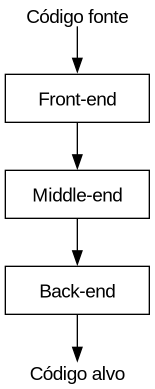
\includegraphics[width=.9\linewidth]{compiler_structure.png}
\label{}
\end{center}
\subsection*{Front-end de um compilador}
\label{sec:orgd1bb5cb}

\begin{itemize}
\item Responsável pela análise do código.
\item Produz uma representação intermediária para geração de código.
\end{itemize}
\subsection*{Middle-end de um compilador}
\label{sec:orgc54cf67}

\begin{itemize}
\item Responsável por otimizações independentes de arquitetura.
\begin{itemize}
\item Constant folding: substituir 3 + 4 por 7 no código.
\item Dead code elimination: eliminar código que nunca é executado.
\item Loop unrolling: eliminar laços para reduzir custo de desvios.
\end{itemize}
\end{itemize}
\subsection*{Back-end de um compilador}
\label{sec:orgcb9e15d}

\begin{itemize}
\item Responsável por otimizações dependentes do hardware.
\begin{itemize}
\item Alocação de registradores: como usar registradores da melhor maneira?
\item Escalonamento de instruções: Decidir ordem de instruções para melhor eficiência?
\item Otimizações específicas de arquitetura: usar vectorização, múltiplos núcleos.
\end{itemize}
\end{itemize}
\subsection*{Porque essa arquitetura?}
\label{sec:org49bd26c}

\begin{itemize}
\item Um mesmo front-end pode suportar diferentes middle-ends, sem modificações na linguagem fonte.
\item Um mesmo middle-end pode suportar diferentes arquiteturas.
\item Separação permite que desenvolvimento seja focado em problemas de cada componente.
\end{itemize}
\subsection*{Exemplos}
\label{sec:org6b7424f}

\begin{center}
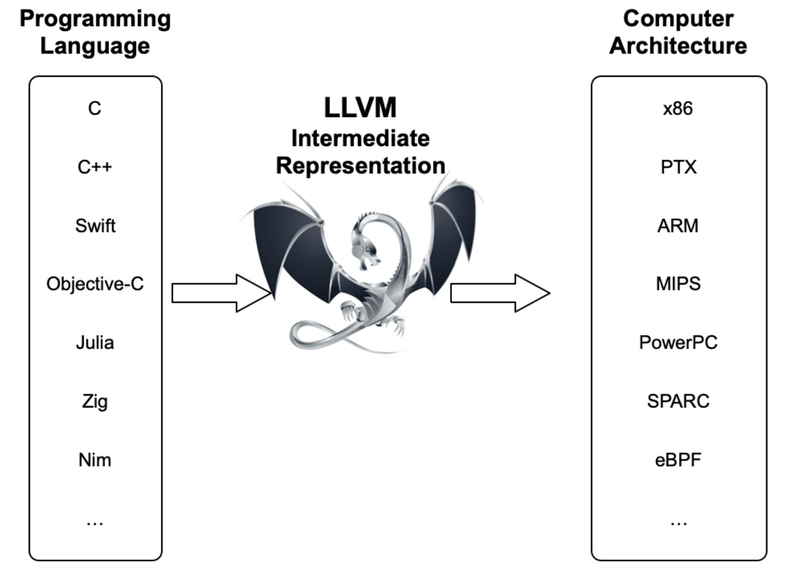
\includegraphics[width=.9\linewidth]{ llvm1.png}
\end{center}
\subsection*{Exemplos}
\label{sec:orgebf449e}

\begin{center}
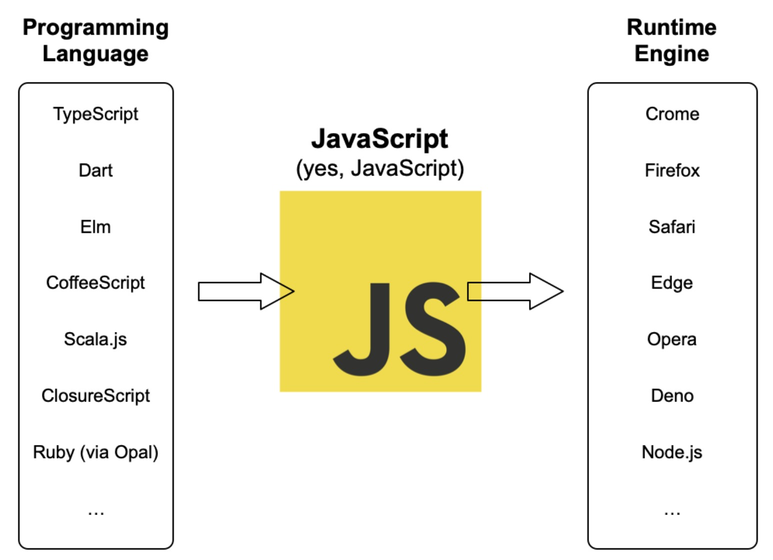
\includegraphics[width=.9\linewidth]{ javascript.png}
\end{center}
\subsection*{Exemplos}
\label{sec:org7f92bd5}

\begin{center}
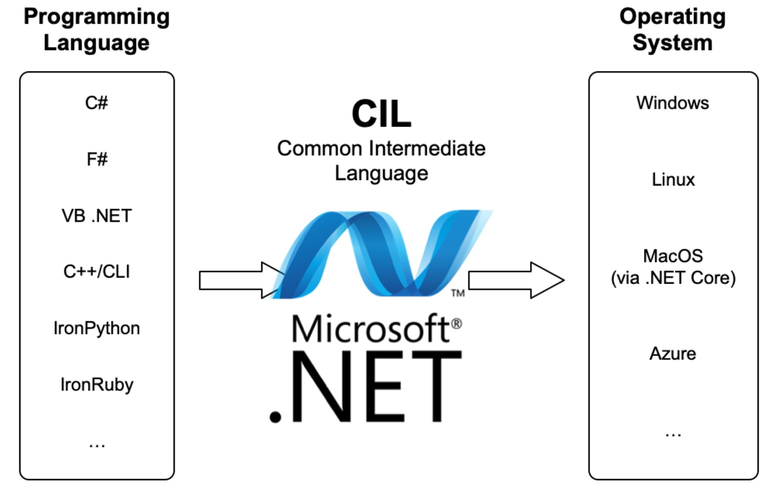
\includegraphics[width=.9\linewidth]{ net.png}
\end{center}
\subsection*{Exemplos}
\label{sec:org3097ee8}

\begin{center}
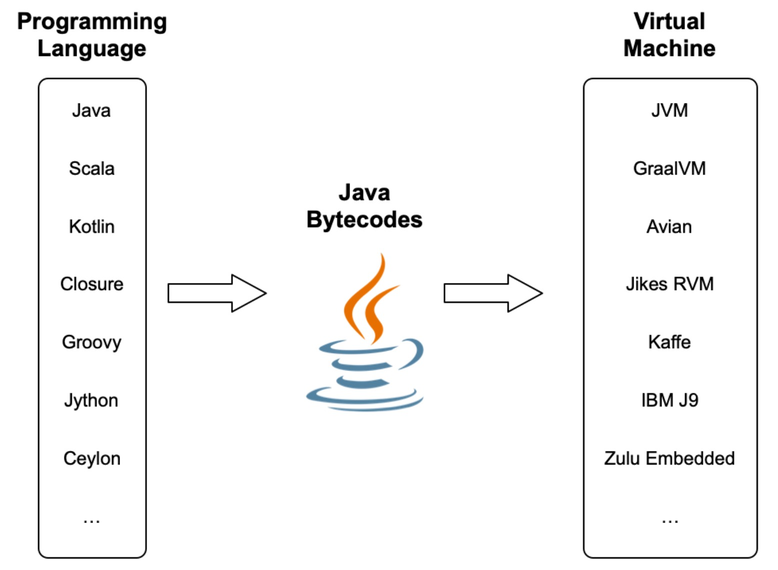
\includegraphics[width=.9\linewidth]{ java.png}
\end{center}
\section*{Ementa}
\label{sec:org6a277b0}

\subsection*{Ementa}
\label{sec:org3a5b173}

\begin{itemize}
\item Introdução ao processo de compilação e interpretação

\item Análise léxica

\item Análise sintática

\item Análise semântica e geração de código intermediário.
\end{itemize}
\section*{Bibliografia}
\label{sec:orgbefdec4}

\subsection*{Bibliografia}
\label{sec:org5e88e19}

\begin{itemize}
\item Construindo Compiladores. Cooper, Keith D. ; Torcson, Linda

\item Compiladores: Princípios, técnicas e ferramentas. Aho, Alfred; Lam,
Monica; Sethi, Ravi; Ullman, Jeffrey.

\item Modern compiler implementation in ML. Appel, Andrew.
\end{itemize}
\section*{Materiais de apoio}
\label{sec:org7fd9e1a}

\subsection*{Materiais de apoio}
\label{sec:orgfdeab99}

\begin{itemize}
\item Slides e código de exemplo serão disponibilizados no seguinte
repositório online.
\end{itemize}
\section*{Critérios de Avaliação}
\label{sec:org82c7bba}

\subsection*{Critérios de Avaliação}
\label{sec:orgdc60792}

\begin{itemize}
\item Uma avaliação no valor de 4,0 pontos.

\item Trabalhos práticos e exercícios de programação no valor 6,0 pontos.
\end{itemize}
\subsection*{Critérios de Avaliação}
\label{sec:org710d82c}

\begin{itemize}
\item Avaliação versa sobre o conteúdo teórico da disciplina:
\begin{itemize}
\item Funcionamento de algoritmos
\item Semântica de linguagens de programação
\item Sistemas de tipos
\end{itemize}
\end{itemize}
\subsection*{Critérios de Avaliação}
\label{sec:orgc9ef4a1}

\begin{itemize}
\item Trabalhos práticos sobre o conteúdo
\begin{itemize}
\item Extensão de protótipos de compiladores apresentados na disciplina.
\item Desenvolvimento de um projeto de ferramenta que utiliza técnicas de
compilação.
\end{itemize}
\end{itemize}
\subsection*{Critérios de Avaliação}
\label{sec:orgdb04819}

\begin{itemize}
\item Entregas de trabalhos
\begin{itemize}
\item Entrega 1: 25/10/2023
\item Entrega 2: 18/11/2023
\item Entrega 3: 29/01/2024
\end{itemize}
\end{itemize}
\subsection*{Critérios de Avaliação}
\label{sec:org1dc6f8e}

\begin{itemize}
\item Exercícios de programação
\begin{itemize}
\item Datas de entrega a serem determinadas na plataforma Moodle.
\end{itemize}
\end{itemize}
\subsection*{Critérios de Avaliação}
\label{sec:org832f3a5}

\begin{itemize}
\item Data avaliação: 05/02/2024
\end{itemize}
\subsection*{Exame especial}
\label{sec:orgc4a2fc7}

\begin{itemize}
\item Mínimo de 75\% de frequência e nota inferior a 6,0.

\item Exame especial parcial para alunos que perderam uma avaliação.

\begin{itemize}
\item Envolverá tarefas de codificação e atividades teóricas (em papel).
\end{itemize}

\item Detalhes: Resolução CEPE 2880 de 05/2006
\end{itemize}
\subsection*{Exame especial}
\label{sec:orgd551ee8}

\begin{itemize}
\item Data do exame especial: 19/02/2024
\end{itemize}
\section*{Software}
\label{sec:orgb17c7fb}

\subsection*{Software}
\label{sec:orgc937e84}

\begin{itemize}
\item Trabalhos e códigos de exemplo serão desenvolvidos utilizando Haskell.

\item Utilizaremos diversas bibliotecas da linguagem Haskell.
\end{itemize}
\section*{Outras informações}
\label{sec:org673e3da}

\subsection*{Informações}
\label{sec:org46dbcd6}

\begin{itemize}
\item Toda informação da disciplina será disponibilizada na plataforma
Moodle.

\item Email: rodrigo.ribeiro@ufop.edu.br
\end{itemize}
\subsection*{Atendimento}
\label{sec:org084d866}

\begin{itemize}
\item Segunda-feira: 08:00 - 10:00h e 15:30-17:30h.
\item Quarta-feira: 08:00 - 10:00h.
\end{itemize}
\subsection*{Finalizando}
\label{sec:org667d57a}

\begin{itemize}
\item Tenhamos todos um excelente semestre de trabalho!
\end{itemize}
\section*{Conclusão}
\label{sec:org4dfb57d}

\subsection*{Conclusão}
\label{sec:orgfcf468b}
\begin{itemize}
\item Próximas aulas: Análise léxica.
\end{itemize}
\section*{Bibliografia}
\label{sec:org910dab1}

\begin{itemize}
\item Compiladores: Princípios, técnicas e ferramentas. Aho, et.al.
\item Crafting interpreters. Nystrom, Robert.
\end{itemize}
\end{document}
